\documentclass[a4paper]{article}

\usepackage[T1]{fontenc}
\usepackage[latin1]{inputenc}
\usepackage{ngerman}
\usepackage{listings}
\usepackage{graphicx}
\renewcommand{\figurename}{Figure}
\usepackage{eso-pic}
\usepackage{pstricks}

\begin{document}

\begin{center}
\textbf{\LARGE{Dresden OCL2 Toolkit Version 2 Tutorial\newline\newline}}
by Ronny Brandt and Claas Wilke
\end{center}

  These tutorial describes the work with the Dresden OCL2 Toolkit version 2. The version 2 is based on the new infrastructure called the ``pivot model"'. The pivot model was developed by Matthias Br�uer and is described in his ``Gro�er Beleg"' \cite{GBBraeuer}. Further information about the toolkit is available at the website of the Dresden OCL2 Toolkit \cite{ToolkitHP}.

	The tutorial starts with the installation of the needed Eclipse plugins. Then it is described how to load a domain specific model and a model instance. Afterwords the importation and interpretation of OCL expressions will be explained.

  The procedure described in this tutorial is realized and tested with Eclipse 3.3.2 \cite{Ecl}. Besides the Eclipse SDK you also need to install the required plugins of the Eclipse Modeling Framework (EMF). During this tutorial the EMF plugins of version 2.3.2 were used.
 
  To install the EMF plugins you have to download them from the EMF website \cite{EMF} and to extract them into the ``plugins"' directory of Eclipse. Afterwords you can start the Eclipse SDK. Alternatively you can install the plugins by using the Eclipse Update Manager after starting the Eclipse SDK.
	
	\section{Installing the Dresden OCL2 Toolkit}
	
	To use the Dresden 0CL2 Toolkit you need to install them as Eclipse plugins, or to import them into your Eclipse workspace. Both possibilities are explained in the following.
	
	\subsection{Installing the Eclipse plugins}
	
	To install the OCL2 Toolkit as Eclipse plugins, you need to have the jar archives of the toolkit. The jar archives are available at \cite{ToolkitSourceforge}. You need to copy the jar archives into the ``plugins"' directory of your Eclipse SDK distribution. Then you can start the Eclipse SDK and you can work with the Toolkit.
	
	\subsection{Importing the Toolkit into an Eclipse Workspace}

	Alternatively you can import the OCL2 Toolkit as plugin projects into an Eclipse workspace. There are two different options to do that.

On the one hand you can import the plugins from your file system, if you already have downloaded them (e.g. from \cite{ToolkitSourceforge} as a source code distribution). One the other hand you can import the plugins directly from the SVN (Subversion) directory of the Dresden OCL2 Toolkit. Both possibilities are described below.
	
	\subsubsection{Import the plugins from the local file system}
	
	Let's say you have the plugins located in a directory \lstinline|XYZ| of your file system. To import them into your Eclipse workspace you can use the Eclipse import wizard. Open the wizard via the menu ``File > Import...`` and select  ``General > Existing Projects into Workspace"' (see figure \ref{pic:Import-EPiW}). In the following window you select the directory \lstinline|XYZ| as root. Then you select the plugins you want to import (if not selected automatically) and activate the check box ``Copy projects into workspace"' (see figure \ref{pic:ImportProjects}). After pressing the button ``Finish"' the plugins will be imported as projects into your workspace.
	
	\begin{figure}[!htbp]
		\centering
		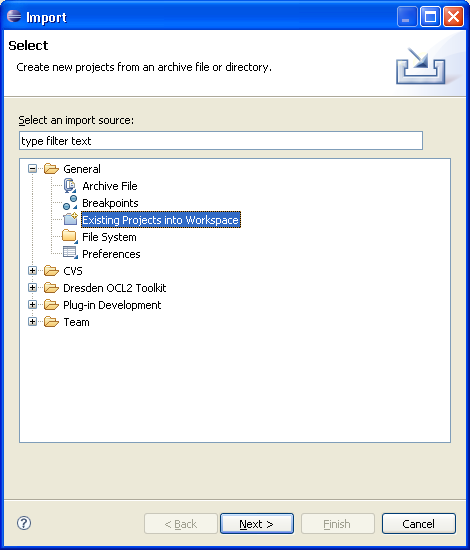
\includegraphics[width=0.8\linewidth]{Bilder/Import-EPiW}
		\caption{Plugin import from local file system (1).}
		\label{pic:Import-EPiW}
	\end{figure}
	
	\begin{figure}[!htbp]
		\centering
		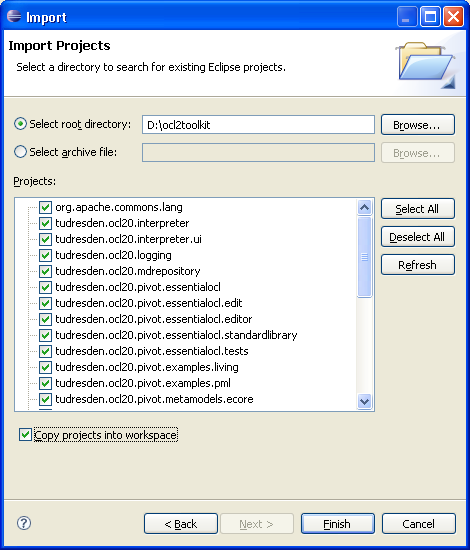
\includegraphics[width=0.8\linewidth]{Bilder/ImportProjects}
		\caption{Plugin import from local file system (2).}
		\label{pic:ImportProjects}
	\end{figure}
	
	\subsubsection{Import the plugin projects from SVN}
	
	To import the plugins directly from the SVN repository, you need to install an additionally Eclipse plugin to connect with the SVN. The needed plugin is called Subclipse (\cite{SVN}). The installation of Subclipse is explained on the Supclipse website \cite{SVNInstall}.
	
  After installing Subclipse a new Eclispe perspective for access to SVN should exist. The perspective can be opened via the menu ``Window > Open Perpective > Other... > SVN Repository Exploring"'. In the view ``SVN Repository"' you can add a new repository (see figure \ref{pic:SVN}) using the URL ``https://dresden-ocl.svn.sourceforge.net/svnroot/dresden-ocl/"'. After pressing the button ``Finish"' the SVN repository root should the visible in the repository view.
	
	To checkout the plugins, you now select them in the repository directory ``trunk/ocl20/eclipse"' and use the ``Checkout..."' function in the context menu (see figure \ref{pic:Checkout}). The given settings could be used and after a click on the ``Finish"' button the plugins should be imported.
	
	\begin{figure}[!htbp]
		\centering
		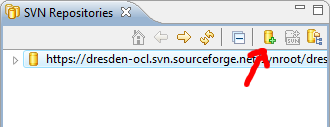
\includegraphics[width=0.5\linewidth]{Bilder/SVN}
		\caption{Adding an SVN repository.}
		\label{pic:SVN}
	\end{figure}
	
	\begin{figure}[!htbp]
		\centering
		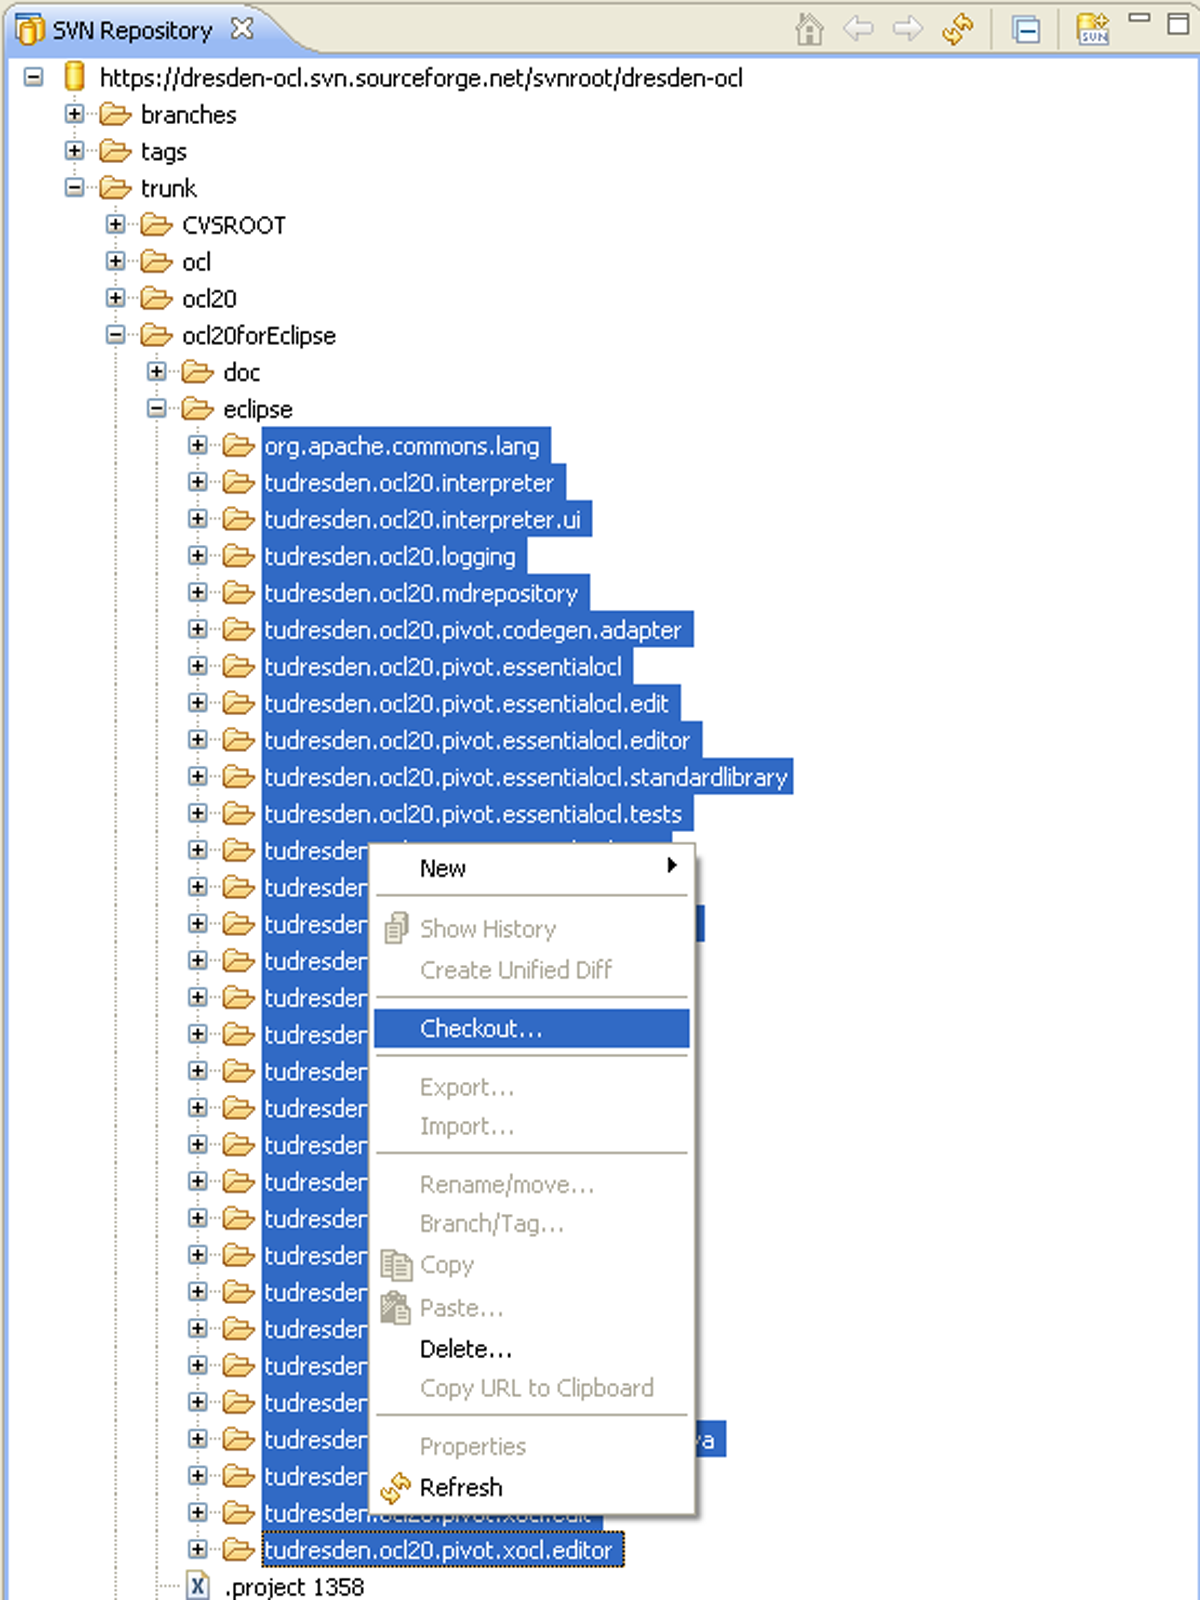
\includegraphics[width=1.0\linewidth]{Bilder/Checkout}
		\caption{Checkout of the Dresden OCL2 Toolkit plugin projects.}
		\label{pic:Checkout}
	\end{figure}

	\section{Building the OCL2 Parser}
	
  If you decided to run the OCL2 Toolkit as project plugins into your workspace,  you need to build the OCL2 parser of the Dresden OCL2 Toolkit via an Ant build script. If you installed the Toolkit using jar archives, you can skip this chapter of the tutorial.
  
  To build the OCL2 Parser select the file ``build.xml"' in the project ``tudresden.ocl20.pivot.ocl2parser"' and open the context menu via a right mouse click. Select the function ``Run As ... > Ant Build"' (see figure \ref{pic:Build}).

	If you decided to run the OCL2 Toolkit as project plugins into your workspace,  you need to build the OCL2 parser of the Dresden OCL2 Toolkt via an Ant build script. If you installed the Toolkit using jar archives, you can skip this chapter of the tutorial.
	To build the OCL2 Parser select the file ``build.xml"' in the project ``tudresden.ocl20.pivot.ocl2parser"' and open the context menu via a right mouse click. Select the function ``Run As ... > Ant Build"' (see figure \ref{pic:Build}).

	\begin{figure}[!htbp]
		\centering
		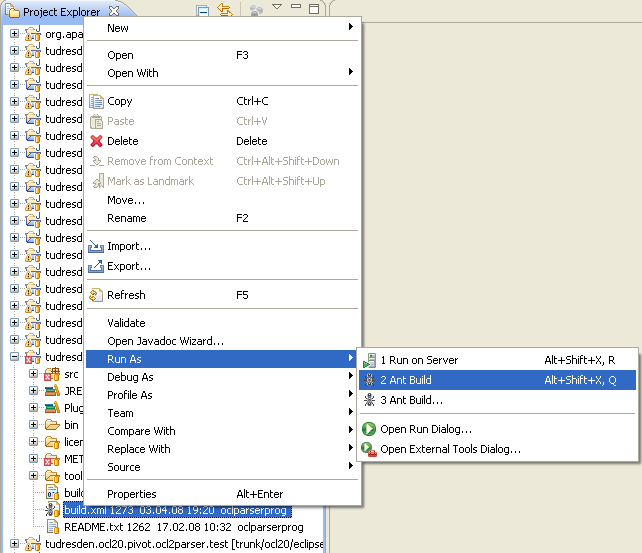
\includegraphics[width=1.0\linewidth]{Bilder/Build}
		\caption{Executing the OCL2 parser build script.}
		\label{pic:Build}
	\end{figure}
	
	If an error like ``Problem: failed to create task or type eclipse.refresh\-Local"' occurs, you need to change the configuration of the Ant script. Open the function ``Properties"' in the context menu of the ``build.xml``. A new window should open. Select the topic ``Run/Debug settings"' and then the configuration for ``tudresden.ocl20.pivot.oclparser build.xml"'. Click on the button ``Edit"'. In the new window select in the sub menu ``JRE"' the check box ``Run in the same JRE as the workspace"' and click on the button ``OK"' (see figure \ref{pic:AntConfig}). Afterwords the Ant script should be executable without errors.
	
	\begin{figure}[!htbp]
		\centering
		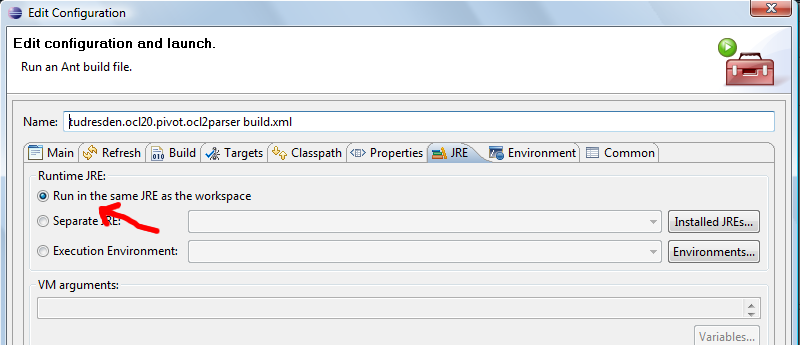
\includegraphics[width=1.0\linewidth]{Bilder/AntConfig}
		\caption{Settings of the JRE for the Ant build script.}
		\label{pic:AntConfig}
	\end{figure}
	
	After executing the build script successfully you need to update the projects in your workspace. Update the project ``tudresden.ocl20.pivot.oclparser"' via context menu (``Refresh"', see figure \ref{pic:Refresh}).

	\begin{figure}[!htbp]
		\centering
		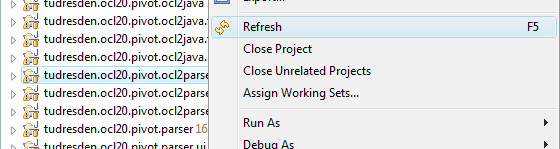
\includegraphics[width=0.5\linewidth]{Bilder/Refresh}
		\caption{Refreshing the project ``tudresden.ocl20.pivot.oclparser"'.}
		\label{pic:Refresh}
	\end{figure}
	
	Additionally you need to recompile all depending projects. Select the function ``Project > Clean... > Clean all projects"' in the Eclipse menu to clean all projects. All the projects should not contain any errors anymore and should be executable.
	
	\section{Using the Dresden OCL2 Toolkit Version 2}

	If you installed the OCL2 Tookit using jar archives, you can execute the Toolkit by starting your Eclipse SDK. If you imported the Toolkit as plugin projects into an Eclispe workspace, you have to start a new Eclipse SDK instance. You can start a new instance via the menu ``Run > Run As > Eclipse Application"'. If the menu ``Eclipse Application"' is not available or disabled you need to select one of the plugins of the toolkit first. After starting the new Eclipse instance you can use the Dresden OCL2 Toolkit as described below.
	
	\subsection{Loading a domain specific model}
	
	After starting the Eclipse instance you have to load a model into the toolkit. You can load a model by using the import wizard (File~>~Import...). Select the wizard ``Dresden OCL2 Toolkit > Domain-Specific~Model"'. In a new opened window you have to select a model file and a meta model for the model (see figure \ref{pic:LoadModel}). During this tutorial the PML Model is used which you can find in the project ``tudresden.ocl20.examples.pml"' in the file ``model/pml.ecore"'.

	\begin{figure}[!htbp]
		\centering
		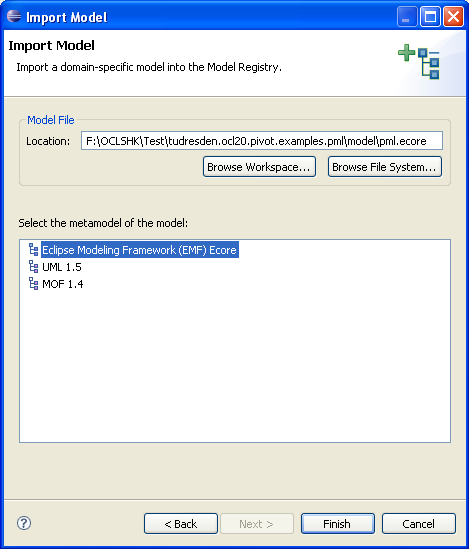
\includegraphics[width=0.8\linewidth]{Bilder/LoadModel}
		\caption{Loading a domain specific model.}
		\label{pic:LoadModel}
	\end{figure}
	
	Figure \ref{pic:MoBrOE} shows the loaded PML model, which uses Ecore as its meta model. Via the menu button (the little triangle in the right top corner) you can switch between different models in the model browser.
	
	\begin{figure}[!htbp]
		\centering
		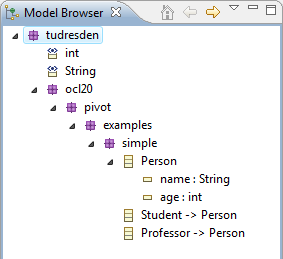
\includegraphics[width=0.5\linewidth]{Bilder/MoBrOE}
		\caption{The loaded PML model in the model browser.}
		\label{pic:MoBrOE}
	\end{figure}
	
	\subsection{Loading a model instance}
	
	After loading the model, you can load a model instance using another import wizard. Use the wizard ``Dresden OCL2 Toolkit > Model Instance"'. You have to select a model instance (in this tutorial we used the file ``model instance/Testmodell.pml"' of the project ``tudresden.ocl20.examples.pml"') and the domain specific model loaded before (see figure \ref{pic:LoadInstance}).

	\begin{figure}[!htbp]
		\centering
		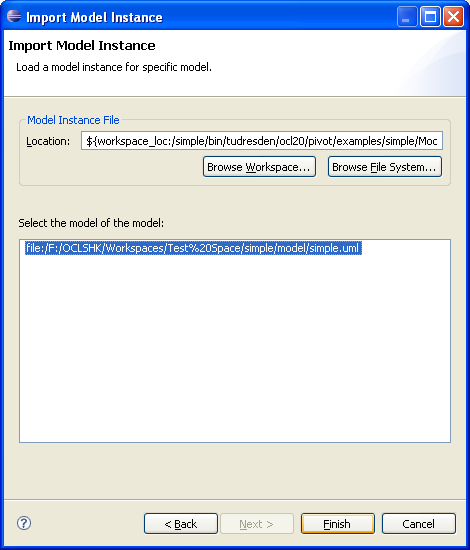
\includegraphics[width=0.8\linewidth]{Bilder/LoadInstance}
		\caption{Loading a PML model instance.}
		\label{pic:LoadInstance}
	\end{figure}
	
	Figure \ref{pic:MoInBr} shows the loaded model instance of the PML model. Like in the model browser you can switch between different model instances. Note that the model instance browser only shows the model instances of the model actually selected in the model browser. By switching the domain specific model, you also switch the pool of model instances available in the model instance browser.
	
	\begin{figure}[!htbp]
		\centering
		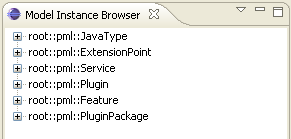
\includegraphics[width=0.5\linewidth]{Bilder/MoInBr}
		\caption{A loaded PML model instance in the Model Instance Browser.}
		\label{pic:MoInBr}
	\end{figure}
	
	\subsection{Loading OCL expressions}
	\indent
	
	Before you can interprete OCL constraints you have to load them like the domain specific model and the model instance before. Use the wizard  ``Dresden OCL2 Toolkit > OCL Expressions"' and select an OCL file (in this tutorial we used the OCL file ``espressions/testpml.ocl"' of the project ``tudresden.ocl20.examples.pml"', see figure \ref{pic:LoadExpressions}).

	\begin{figure}[!htbp]
		\centering
		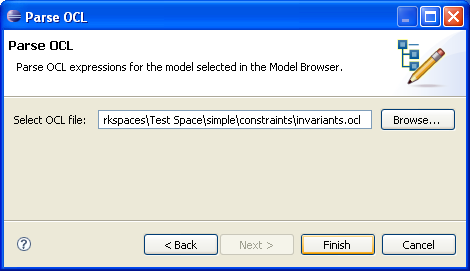
\includegraphics[width=0.8\linewidth]{Bilder/LoadExpressions}
		\caption{The import of OCL expressions of a model loaded before.}
		\label{pic:LoadExpressions}
	\end{figure}
	
	The expressions of the selected OCL file will be loaded into the actually selected model instance. Figure \ref{pic:MoBrME} shows the  ``Model~Browser"' containing the PML model and the parsed expressions.
	
	\begin{figure}[!htbp]
		\centering
		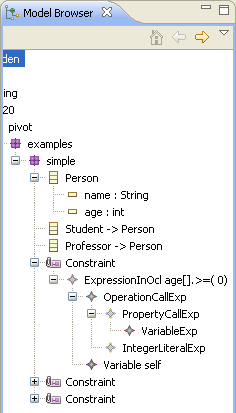
\includegraphics[width=0.5\linewidth]{Bilder/MoBrME}
		\caption{Parsed expressions of the PML model in the Model Browser.}
		\label{pic:MoBrME}
	\end{figure}
	
	\subsection{Interpretation of constraints}
	\indent
	
	The interpretation of constraints is possible via the Interpreter View. The view provides a context menu containing all needed functionality. The context menu is shown in figure \ref{pic:IntViewMen} (You can open the context menu via the little triangle in the right top corner of the Interpreter View).
	
	\begin{figure}[!htbp]
		\centering
		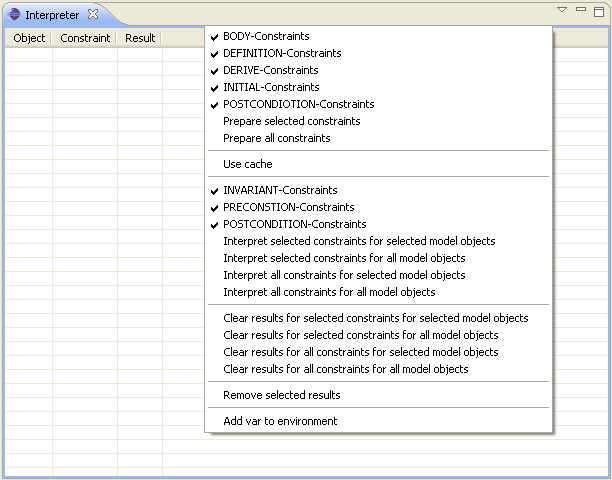
\includegraphics[width=1\linewidth]{Bilder/IntViewMen}
		\caption{The context menu of the Tnterpreter View}
		\label{pic:IntViewMen}
	\end{figure}
	
	For the interpretation of constraints you can use the functions ``Interpret~..."' in the context menu. First you can select constraints you want to interpret in the ``Model~Browser"' and the model objects for which the constraints should be interpreted in the ``Model~Instance~Browser"'. The ``Model~Instance~Browser"' shows only the model objects, for which you can interpret the constraints selected before.
	
	In the interpreter menu you can select the types you want to interpret (invariants, pre and post conditions). After interpretation the table in the Interpreter View shows all results. These are filtered by the selection of constraints and model objects. Figure \ref{pic:IntView} shows a table with some results. If the column ``Result"' does not contain enough space for a result, you can open a result via a double mouse click in a new window.
	
	\begin{figure}[!htbp]
		\centering
		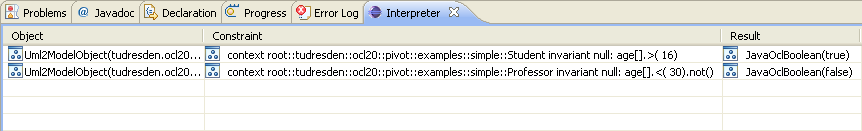
\includegraphics[width=1\linewidth]{Bilder/IntView}
		\caption{Some results in the Interpreter View.}
		\label{pic:IntView}
	\end{figure}
	
	\subsection{Additional functionality of the interpreter}
	
	Before interpretation you can prepare some or all constraints like described in \cite[Abschnitt Environment]{DABrandt} (``Prepare~..."').
	
	You can add variables to the \lstinline|environment| via ``Add~var~to~environment"'. This functionality can be used for parameters and results of operations or the name of parameters. Figure \ref{pic:AVTEnv} shows a window to add variables to the environment. After entering a variable name (e.g. ``result"' or the name of a parameter) a primitive type object (e.g. Integer) can be created or the result of an already interpreted constraint can be used.
	
	\begin{figure}[!htbp]
		\centering
		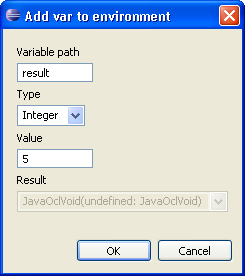
\includegraphics[width=0.4\linewidth]{Bilder/AVTEnv}
		\caption{Window to add a variable to the environment.}
		\label{pic:AVTEnv}
	\end{figure}
	
	Using the ``Clear~..."' functionality, results can be removed from the interpreter view. You can remove all results or select results which you want to remove before (``Remove~Selected~Results"').
	
  Using the check box ``Use~cache"', you can activate the caching mechanism described in \cite{DABrandt} to improve the performance of the interpreter.
  
  \section{Conclusion}
  
  This tutorial described how to use the Dresden OCL2 Toolkit version 2. It explained how to install or import and start the Toolkit's plugins. Afterwards the usage of the interpreter of the Dresden OCL2 Toolkit was shown.
  	
	As mentioned before, more information about the Dresden OCL2 Toolkit is available at the website of Dresden OCL2 Toolkits \cite{ToolkitHP}.

	\newpage
	\bibliographystyle{alphadin}
	\bibliography{literature}

\end{document}
